\documentclass[11pt, oneside]{article}   	% use "amsart" instead of "article" for AMSLaTeX format
\usepackage{geometry}                		% See geometry.pdf to learn the layout options. There are lots.
\geometry{letterpaper}                   		% ... or a4paper or a5paper or ... 
%\geometry{landscape}                		% Activate for rotated page geometry
%\usepackage[parfill]{parskip}    		% Activate to begin paragraphs with an empty line rather than an indent
\usepackage{graphicx}				% Use pdf, png, jpg, or eps§ with pdflatex; use eps in DVI mode
								% TeX will automatically convert eps --> pdf in pdflatex		


%SetFonts

%SetFonts
%\usepackage{tikz}
%\usepackage{amsmath}	
%\usepackage{amssymb}
%\usepackage{xcolor}
%\usepackage{url}

%\usepackage[official]{eurosym}
%\usepackage{multicol}
%\usepackage{wasysym}

%\usepackage{academicons}
%\usepackage{dtklogos}
%\usepackage{braket}
%\usepackage{bm}
%\usepackage[utf8x]{inputenc}
%\usepackage{natbib}
\usepackage{multicol}
\usepackage{graphicx}
\usepackage{amssymb}
\usepackage{amsmath}
\usepackage{braket}
\usepackage{tikz}
\usepackage{pgfplots}
\pgfplotsset{compat=1.10}
\usepackage{filecontents}
%\usepackage{hyperref}
\usepackage{url}
\usepackage[makeroom]{cancel}
\usepackage{turnstile}
\usepackage[hypcap]{caption}
\usetikzlibrary{bayesnet}
\usetikzlibrary{positioning, arrows, decorations.markings, matrix, decorations}
\newcommand{\peh}{P(E|H)}
\newcommand{\phe}{P(H|E)}
\newcommand{\ph}{P(H)}
\newcommand{\pe}{P(E)}
\def\ci{\perp\!\!\!\perp}
\usepackage{amsthm}
\usepackage{bussproofs}
\EnableBpAbbreviations
\newcommand{\seq}{\Rightarrow}
\newcommand{\imp}{\rightarrow}
\newcommand{\bico}{\leftrightarrow}
\newcommand{\RLab}{\RightLabel}
\newcommand{\LLab}{\LeftLabel}
\newcommand{\logicname}{QMC}
\newcommand{\qax}{\ket{0} \seq}
\newcommand{\hadz}{\frac{1}{\sqrt{2}}\ket{0} + \frac{1}{\sqrt{2}}\ket{1}}
%\usetikzlibrary{positioning,arrows,decorations}
\usepackage{relsize}
%\usepackage[greek]{babel}
%\usepackage{amsfonts}
%\usepackage[utf8x]{inputenc}


\usetikzlibrary{bayesnet}
\usetikzlibrary{arrows, decorations.markings, matrix, decorations.pathmorphing}
\usetikzlibrary{decorations.pathreplacing}

\DeclareMathOperator{\graphrightarrow}{\tikz[baseline=-0.8ex]{ \draw [scale=1,->] (0,0) -- (4ex,0); }}
	\DeclareMathOperator{\graphleftarrow}{\tikz[baseline=-0.8ex]{ \draw [scale=1,<-] (0,0) -- (4ex,0); }}
	\DeclareMathOperator{\graphcontour}{\tikz[baseline=-0.8ex]{ \draw [scale=1,-] (0,0) -- (3ex,0); }}

	\DeclareMathAlphabet{\mathpzc}{OT1}{pzc}{m}{it}

\newenvironment{definition}[1][Definition]{\begin{trivlist}
\item[\hskip \labelsep {\bfseries #1}]}{\end{trivlist}}









\usepackage{mathrsfs}
\usepackage{lmodern}
\usepackage[T1]{fontenc} % Output font encoding for international characters
%\usepackage{natbib}










\sloppy
%\newtheorem{definition}{Definition}
\newtheorem{theorem}{Definition}


\usepackage{hyperref}
\usepackage{fontawesome5}
\usepackage[natbibapa,nodoi]{apacite}



\hypersetup{
    colorlinks = true,
    %linkbordercolor = {blue},
    linkcolor = {black},
    urlcolor = {blue},
    urlbordercolor = {blue},
    citecolor = {blue},
}

%\newtheorem{theorem}{Definition}

\setcounter{secnumdepth}{-2}

\title{AI/ML Experience and Research Plan}
\author{Cameron Beebe, Ph.D.}
%\date{}							% Activate to display a given date or no date

\begin{document}
\maketitle
%\section{}
%\subsection{}




\noindent This document provides a brief overview of my research experience and associated projects in AI, both practical and theoretical.  I have emphasized where relevant to reinforcement learning and explanation.  I have attached some excerpts from my written work and some brief commentary where appropriate to explain technical points.  The full context is available in online repositories of my projects,  papers, and dissertation.  


\tableofcontents

\section{Methodology}

\begin{itemize}
    \item \textbf{Large Language Models.}  I swear I will \textbf{not} use LLMs to summarize literature, write text for my papers, or to help construct ``novel'' arguments or substitute for my own effort and cognition in any way. Any use will be purely for research purposes of what they are capable of. 
    \item \textbf{Transparent Research.}  I can and will use Git version control for my projects, and host them in GitHub repositories for transparency.  (See e.g. \href{https://github.com/CameronBeebe/Structural_Idealism}{Structural Idealism Project}.) 
    \item \textbf{Networking.} I spent almost a decade associated with the Munich Center for Mathematical Philosophy.  I am also working on a project in philosophy of physics as an external member.  I created The SciPhi Initiative, LLC, and have used this organization for tutoring and outreach.  I will continue to use social media, primarily those where tech and AI industry experts are also present, to engage with respect to research and ethics goals.
    \item \textbf{Interdisciplinary.}  I value very much interdisciplinary collaboration, and this has been a major characteristic of my previous academic experience at the Munich Center for Mathematical Philosophy and Graduate School of Systemic Neurosciences.
    \item \textbf{Inclusive.}  I want to discuss diverse points of view on these topics.  See e.g. the convincing arguments from John Stuart Mill's \emph{On Liberty} for considering in particular voices less heard.
    \item \textbf{Belief Revision.}  I will revise my beliefs and research goals as compelling new information is presented to me, within the scope of the project.
    \item \textbf{Historical Synthesis}.  There is a lot of work (which predates widespread LLM availability) which deserves attention, critical analysis, and potential synthesis with newer work in AI.
    
\end{itemize}







\section{Two Main Projects}


\subsection{Machine Epistemology and Ramsey Sentences}

Is it possible that an AI model could learn a different structural representation of the world compared to a typical human biological neural net, and we won’t be able to tell?  If we are going to use artificial generative models in science, what is the epistemological character of apparently new scientific information which is derived from such models?  Assuming it is plausible to suppose some kind of a divide between empirical and theoretical terms, can new information derived from generative AI ever go beyond what philosophers of science call \emph{empirical structural realism}?

A neural network model can learn "empirical" laws which generalize the model's ``environment''.  We can say that the model learns an effective bias. That environment is not the same as the one humans like you and I inhabit.   We might suppose, however, that the training data encodes sufficient similarities to our own world.  Sufficient for the model to learn essentially isomorphic empirical laws to our own reality.

A major follow up question is whether the model can learn the same or new \emph{theoretical} laws to our own.  In our explanations of the world we use theoretical laws, which can include potentially non-observable theoretical terms.  They are essential to our cognition of the world.  I think it is extremely unclear whether we should expect current AI models to truly learn anything like our theoretical laws (although they might mimic quite well or be pre-prompted to give the illusion that they understand them).  

To truly ``learn'' theoretical laws from scratch, what would the training data need to look like, and how do mechanisms in the model "digest" the data?  If we found something which looked like a new theoretical law in the architecture or output of a model, how would we evaluate it?  What tests could we do to find out whether a model has learned different theoretical laws from our own, or new ones?  Would it matter, if the empirical laws remained isomorphic?

Ramsey sentences attempt to do without theoretical terms, so perhaps we could coordinate the machine's epistemology with our own through such a formalization.  

See e.g. \citep[\S 26]{Carnap1966} 


% \subsection{Relating Learned Structures to Real Structures}

% Helmholtz, Eddington, etc.

% Do effective structures learned correspond to mere adaptive exploits, or actual (causal) world models.  Clearly, absent strong evidence, we should prefer the former.  However, it isn't clear from a complex systems theory point of view what the actual difference would be.

% However, when we consider the phenomenological and idealist views of philosophy, some might think we smuggle back in human specialness, yet I think we should also consider that the real difference can just be understood as knowledge of the scope of different phenomenal worlds. [??]  Different environmental data distributions to adapt to.  

% This is taking the ontology and epistemology of these systems very seriously, just as we would with other creatures. We seem to be able to specify, with a fairly convincing degree of justification, what the environmental data would be like for ants.  

% But, what about silicon hardware implementing linear algebra circuits? [DOES THAT MAKE SENSE?]

\subsection{A Methodology for Generative Confounds and the Trajectory of Science}

%After more than a decade of widespread social media use, we now have some idea how populations of humans can be affected by algorithmic content pushing.  The algorithms are driven by feedback loops on an industrial scale.  Supercomputers (petascale and, now, exascale) are employed in order to do large amounts of mathematics (conventionally matrix multiplication on forward passes and the chain rule backpropagating feedback signals) in the optimization process.  The information contained in the reinforcing signals from large populations of human consumption allows social media companies to adjust their algorithms, and make them more optimal with respect to the goal of keeping users neurochemically hooked and coming back for more content, and to serve more ads.  

%Increasingly, however, social media companies are ostensibly trying to introduce what I think can be appropriately called \emph{nudges}, in consistent terminological usage with the theory of nudging as put forth in Sunstein et al.  The overwhelming criticism and pushback these companies receive when hateful content or misinformation is algorithmically pushed is almost universal.  Facebook, for example, has employed \emph{tens of thousands} of employees to try to manually flag and determine what should or should not be pushed, in what seems an obvious attempt to create a labeled dataset to train algorithmic content moderation models.

%My understanding of nudging which I think seems fair goes something like this: when all fair choices are presented to an agent (including the ``right'' choice according to some economic or political theory) the probability of the specific (theory-desired) choice might increase at the population level.  This is called ``choice architecture'', and I take it to be an ideal formulation like other theoretical frameworks in economics or related sciences.  

%One problem with algorithmically implementing such an idea is not just that the programmers of the algorithm may have implicit bias (which may or may not agree with the user's implicit bias).  This would, for example, affect the space of choices in certain ways.  However, a much more problematic issue I take to be that users are already in a vulnerable state, being targeted for their attention via the content optimization loop, and therefore susceptible to two kinds of cognitive responses.  

%\noindent\textbf{Positive:} \emph{uncritically believing in the implicit biases of the choice architects as a worldview, which we can perhaps view as a form of confirmation bias}.

%\noindent\textbf{Negative:} \emph{believing that the choice architects are maliciously projecting their world view (which clashes with the user's)}

%[nonsense?]

%I would compare this to 

There are many examples of beneficial uses and properly applied machine learning and artificial intelligence techniques in science.  [EXAMPLES: Predicting turbulent flow, protein structures, ]  It even seems uncontroversial that some of these models can indeed produce new knowledge.  [CITE FUNSEARCH]  The FunSearch results even arguably provide a form of explanation that philosophers of science might recognize.  Previously, I have argued that explanations must be able to intersubjectively transfer the capacity to control.  In the case of FunSearch, the mathematical result which was obtained was at least communicable in the form of a (low $K$ complexity!) program. The mathematical results are impressive, especially if they transfer to other areas of computation and mathematics (e.g. perhaps learning compact low $K$ representations of trained models) but arguably a long way to go from there to new theories and mechanistic explanations in other areas of science.  

\begin{quote}
    What’s more, this interpretability of FunSearch’s programs can provide actionable insights to researchers. As we used FunSearch we noticed, for example, intriguing symmetries in the code of some of its high-scoring outputs. This gave us a new insight into the problem, and we used this insight to refine the problem introduced to FunSearch, resulting in even better solutions. We see this as an exemplar for a collaborative procedure between humans and FunSearch across many problems in mathematics.

    [CITE]
\end{quote}

This is a dialectical relationship to an AI model, which is arguably lacking from the current typical use of widespread models like ChatGPT, which seem to be used more like authoritative Oracles.

The authors note that when FunSearch discovered a much better solution to bin packing compared to traditional heuristics, is easy to check and verify that it is indeed better.  This is exactly like the traditional framing in computational complexity theory, but \emph{what are the complexity requirements for testing scientific claims from generative models?}  Assuming we can determine the claims \emph{are testable}.  For example, claims concerning fundamental physics seem likely to require much more resources than claims about material science.

I think philosophers should take great interest in this novel result, and I argue that we can understand such a result stemming from \emph{dialectical} features of the models.  Novel dialectical architectures should be pursued not just for the potential for justifiability and explainability of alleged new scientific knowledge, but also for reasons of trust and convergence.  Perhaps most importantly, however, I argue that a dialectical architecture has the potential to improve the layman's individual use of generative models.  Rather than LLMs being treated like Oracles, they should be interacted with as if they were \emph{philosophical interlocutors}.  

The epistemological relationship is beneficial because it facilitates critical thinking methods like the Socratic method, rather than a dependency on something akin to confabulatory divination.  

One example of what I would classify as a dialectical model is what is known as an adversarial model. Adversarial models in the past (e.g. Generative Adversarial Models, or GANs) relied on a neural network architecture which pitted one ``sub-network'' against another.  One was typically called a Generator, and a Discriminator.  This can be used for example to learn an image model that reproduces images close to a training set.  The whole system functions in an iterative loop, such that a Generator tries to fool the Discriminator, and the information of ``failure-to-fool'' is fed back to improve the Generator.  The back-and-forth tension is a reliable feedback loop mechanism.

I think that we should explore other forms of architecture for dialectical models, in which the internal ``competition'' among sub-nets is composed differently, and not necessarily competitive or describable as ``fooling''.  Rather, sub-nets try to compose the best argument, and other sub-nets try to poke holes.  Importantly, as similar to the communicability part of FunSearch, such artificial systems should \emph{transparently display the dialectic between ``adversarial'' sub-nets}.  

Hierarchical dialectical models represents a potentially novel architecture which I would expect to find in a successful AGI candidate.  If we are going to have AGI, we should try to engineer an architecture which not only out-competes available alternatives, but does so in a theoretically responsible way.  Naturally, what I am describing represents many potential open problems in need of solution, and I am merely speculating that (open source) development on HDMs would be more responsible than other approaches being developed in the open or in secret.  There is the possibility that AGI is dangerous no matter the architecture, and I find it likely we will have multiple competing models.

I was not the first to note the similar structure of a GAN with the philosophical notion of a dialectic.  [CITE ]

%So, on Oracular calls to the composed network, a dialectic is displayed.  Additionally, one should be able to call upon a ``committee'', and the function of the model is not general but specific to a critical methodology.  






However, for quite some time now, I have been concerned with what I would call \emph{systemic confounds} from generative AI models.  These confounds are present in the results shown from popular search engines, for example ChatGPT output text copied and pasted onto popular forums like StackOverflow and Reddit, and shown by Google search.  This is the obvious ``pollution'' confound, but I believe there are much more important confounds from generative models we should focus on for the methodology of science.



Social media content optimization algorithms have for some time now affected large populations of humans.  Even small changes in content, distributed widely, are expected to potentially affect the views of individuals within the population.  I think it is fair to consider in a similar context a new class of public-facing \emph{generative} algorithms.  The most widely known is OpenAI's large language model (LLM) called ChatGPT.

With the advent and widespread availability and use of generative LLMs, there is now a new optimization loop which reinforces through human feedback a different class of models.  These models aren't necessarily optimized in order to serve content, but to create linguistic content that satisfies in some way a population of human users.  A computation arms race is rapidly increasing the dedicated and specialized compute to training and improving these models, and also to serve artificial linguistic content to large populations of humans.








Consider a phase space, in which each point represents the total state of every human with agency, and every relevant factor of human civilization.  This complex system has, and will have, a \emph{trajectory} in phase space.  There might be ``peaks'' and ``valleys'' in this space, which represent the grain or currents that characterize in summary things like incentives and disincentives, positive and negative feedback loops, and structural constraints in the world of the system.



In a preprint manuscript, Atoosa Kasirzadeh makes a very similar and related point she calls the \emph{accumulative} risk of AI. \citep{Kasirzadeh2024WIP}  It seems to me that central to this accumulative risk is the relationship populations of humans have to widely available generative artificial systems.  Small mistakes and misuses can add up: 

\begin{itemize}
    \item bugs in automatically generated code
    \item relying on generated summaries of articles never read
    \item using generated text in scientific articles
    \item using them to influence ``novel'' scientific theory or results at the fringe of a particular scientist's understanding or, worse, 
    \item at the fringe of a majority of a field's understanding---in which case, an error may persist for quite some time
\end{itemize}

So, if we want to foster \emph{resilience}, it seems to me that we need to focus on making resilient individuals, since they are presumably the smallest ``unit'' or subsystem relevant to the coherent functioning of an interconnected global complex system.  The more resilient individuals, the more robust will be larger subsystems like local organizations and municipalities.

Furthermore, it seems obvious that some networks of individuals (and associated institutions) are more influential and capable of being robust.  Namely, scientific networks and institutions.  These are the networks with individuals most likely to have developed critical thinking skills able to resist poor usage of AI models.  Unfortunately, the current trend looks poor, as scientists (with certain incentives) appear to be among the first and most frequent users of novel AI models, in particular generative language models.

What philosophical views do scientists and developers have, and what epistemological assumptions do they make about AI models?  When one reads, for example, the scientific treatises of some of the smartest people of the twentieth century, there is an astonishing amount of philosophical sophistication.  Much of this has to do with the educational system in Germany and Austria.  But the point is that \emph{it is popular for scientists to forego the philosophy in favor of results and publication}.  The incentives make it so.

Atoosa also suggests simulations and modeling of the complex global system, which I wholeheartedly endorse and would like to explore as well.  




\section{Potential Related Projects}

\subsection{AI Nudges}

\noindent\textbf{What effect might widespread AI nudges have on the trajectory of civilization?}

%Also, if these models are based on human data with questionable privacy protections in the first place, nudges from such a model arguably represent a potential further privacy intervention on distilled data from the population.

Of course, humans are not perfect, and make many of the same mistakes.  Then the epistemological responsibility is still on the humans and their values, rather than dependent on an external and mysterious artificial system.

\textbf{Important Literature:} Nudging (E.g. Sunstein and Thaler, Kapsner and Sandfuchs, )


\subsection{Focus on Bias}

There is a large amount of literature about bias in artificial neural network models.  However, in my opinion this literature focuses mainly on the ethics and corrective procedures in order to balance bias (or even remove the bias totally, which under some  understanding, e.g. that of \citep{Mitchell1980}, is not particularly plausible), which I think is missing a much larger potential issue that tech and AI ethicists should be aware of.  

Even if everyone agreed on criteria for an ``unbiased'' model, and everyone agreed to use it, there are fundamental epistemological limitations about whether we will be able to understand when the models are confabulating or nudging in nuanced ways that affect influential actors in society, which in turn affect the trajectory of science or politics in our civilization.


\subsection{The Viability of Watermarking}

On the issue of a polluted epistemological landscape, will we have to rely on AI tools just to know what is real?  Is there a method, such as watermarking, which could not just be required but actually adhered to?

I think the possibility of reliable and ubiquitous watermarking is extremely unlikely to happen.


\subsection{Scaling and the VC Dimension}

Many papers on scale in neural networks.  Some believe indefinite scaling returns.  I think we can consider the VC dimension to make a strong argument that there will be an eventual plateau of diminishing returns.  Where those diminishing returns might happen is an interesting question.  Some think we are already there.




\subsection{Dialectical Models (Adversarial)}

Many important works in the history of philosophy are dialectical.  The Socratic method is dialectical.  Dialogues are structured arguments between protagonists and antagonists.  The biased interlocutors are engaged in a feedback loop which aims towards a resolution.  

If humans interact with generative models like LLMs as if they are AI Oracles, they become more of a passive part of a  knowledge feedback loop.  Like lazily asking a teacher for the answer to a question, where effort and critical thinking and agency in the world would lead to a more satisfying embodied answer.  Reading a book and doing research and engaging one's own biological neural network has e.g. neural, neuro-chemical, and emotional value above and beyond the critical thinking skills as well.

Not to mention that AI Oracles which crawl the internet for answers are encountering a more polluted environment as they try to find seemingly authoritative and genuine facts.  Generative models, and human agents who are proliferating their outputs, are polluting the very data set which would make them useful long term.  Consider an analogy with \textbf{a microphone getting too close to a speaker.}  Garbage in, garbage out.

While much of this seems obvious to me after a great deal of thought the last few years, I'd be interested in hearing counterarguments.  These models aren't going away anytime soon, and banning them will not work as open source models are proliferated and competitive with closed source ones.  

\textbf{I think it would be worthwhile to explore whether we might be able to develop an alternative kind of generative model which encourages non-Oracle use and critical thinking by the human user.  It outputs considered dialectic from multiple biased models.} \\

\textbf{POTENTIAL CRITICISM}: One can ask current models to simulate a dialectic, or just fine tune on philosophical dialogue texts, so would we really need some new architecture for specifically dialectical models?

\textbf{POTENTIAL RESPONSE}: There is no free lunch.  \cite{Wolpertetal1997}  Effective models learn bias.  \cite{Mitchell1980}  Maybe even some computational efficiency to go down the route of a cluster of adversarial and biased models.  They might also be able to be distributed better on compute devices. 




\subsection{Ethical LLM Usage in Science}

We need to develop checks and balances, proper-use directives, and standard operating procedures for the use of generative language models in science.

Discussing a recent interesting case of a student who (mis-)used LLM models in their work\footnote{\href{https://twitter.com/BeebsMemes/status/1759282741680443600}{Post on X}}:

Perhaps using translation specific language models should be allowed under certain guidelines, especially ones vetted and known to be robust by scientific administrators. So students can write in their comfortable native tongue… and there would be less likelihood of spurious or incoherent content being introduced into the academic process.

But this sidesteps the more fundamental  issue which is that critical thinking skills in human neural nets are atrophying as people become dependent.  I think this student should \emph{not} have used the LLM to rewrite anything, especially if it was something they were unsure about in a second language to begin with. 

As long as there was an affidavit of human authorship, and/or affidavit of translation only (e.g. according to model and version \#), I think it would have been an arguably okay use of AI tools for academic work. But anything above translation gets very suspect, for reasons having to do with the human values of science and the goal to train critical human thinkers in academia.

There is a new and extremely dominant influence in academia, and incentives to empower that influence will lead to outcomes inconsistent with the purpose of higher education if we don’t start figuring out healthy ways to use the technology.



\subsection{Consulting AI Oracles}

If large language models are trained on human data, we are fairly justified in suspecting that the models might encode not just grammar rules and nuances of vocabulary use cases, but also common beliefs about the world.  

Furthermore, the way they are prompted (including system or guard-rail prompts) provides ``divination'' context for the consultant.

\begin{quote}
    But to satisfy the conditions of the problem, the opponents of the great thinker should have penetrated very deeply into the nature of reason, so far as it is concerned with pure thought---a task which did not suit them.  They found a more convenient method of being defiant without any insight, viz., the appeal to \emph{common sense}.  It is indeed a great gift of heaven to possess right or (as they now call it) plain common sense.  But this common sense must be shown in deeds by well-considered and reasonable thoughts and words, not by appealing to it as an oracle when no rational justification of oneself can be advanced.  To appeal to common sense when insight and science fail, and no sooner---this is one of the subtle discoveries of modern times, by means of which the most superficial ranter can safely enter the lists with the most thorough thinker and hold his own.  But as long as a particle of insight remains, no one would think of having recourse to this subterfuge.  Seen in a clear light, it is but an appeal to the opinion of the multitude, of whose applause the philosopher is ashamed, while the popular charlatan glories and confides in it.

    \citep[p. 5]{KantProlegomena}
\end{quote}


Chapter 4 in divination book


\subsection{What to Worry About}

I agree with e.g. Anil Seth and many others when I have \emph{extreme} doubt about any sort of sentience or consciousness in mathematical models implemented on exascale supercomputers.  Given a distribution over possible things to worry about with respect to artificial intelligence, it should be low priority to think about if/whether/when these models might .

Rather, we should focus more on how humans interact with these models.  Turing Tests are best understood as a measure of the ability of an artificial model to \emph{trick} humans.  Modern models, like LLMs, are trained not just on a data set, but refined through reinforcement learning from human feedback. In some very real sense, many of these models are reinforced to impress both individual humans as well as populations of humans.  \textbf{Thumbs up!}







\section{Dissertation: Knowledge Transfer in Cognitive Systems}

\noindent \textbf{Dissertation link:} \href{https://edoc.ub.uni-muenchen.de/28655/}{Knowledge Transfer in Cognitive Systems Theory: Models, Computation, and Explanation} \\

\noindent I argue in my dissertation that we can use Ashby's cybernetics to provide accessible \textbf{explanations} for the kinds of things that artificial neural networks do, as they can be understood as cybernetic regulators.  They are error-controlled feedback systems  \\

\noindent \textbf{Reinforcement Learning can be understood as a form of feedback in a cybernetic regulator.} \\


\noindent Here is the abstract from my dissertation:\\

\noindent \textbf{Abstract:} Knowledge transfer in cognitive systems can be explicated in terms of structure mapping and control.  The structure of an effective model enables adaptive control for the system's intended domain of application.  Knowledge is transferred by a system when control of a new domain is enabled by mapping the structure of a previously effective model.  I advocate for a model-based view of computation which recognizes effective structure mapping at a low level.  Artificial neural network systems are furthermore viewed as model-based, where effective models are learned through feedback.  Thus, many of the most popular artificial neural network systems are best understood in light of the cybernetic tradition as error-controlled regulators.  Knowledge transfer with pre-trained networks (transfer learning) can, when automated like other machine learning methods, be seen as an advancement towards artificial general intelligence.  I argue this is convincing because it is akin to automating a general systems methodology of knowledge transfer in scientific reasoning.  Analogical reasoning is typical in such a methodology, and some accounts view analogical cognition as the core of cognition which provides adaptive benefits through efficient knowledge transfer.


\subsection{EXCERPT: Ashby on Knowledge as Control}

\noindent \textbf{Knowledge transfer is explicated as the effective transfer of control.}\\

The conception of knowledge most relevant to the topic of this dissertation is that of control.  Knowledge is nothing more than the ability to control a system.  While there might be some other sense of knowledge which doesn't need to exhibit control, it may be of little use for scientists.  Demonstrating control is a part of experimentation, explanation, and a scientific methodology.  I outline this view by citing specific passages in W. Ross Ashby's journal compilation, where he makes it explicitly clear.  As I find these passages to be not only informative on the subject of the dissertation as well as historically interesting, I quote these passages at length here, and occasionally throughout.\footnote{Ashby's digital journal collection is extensively cross-referenced by keywords.  It could be that some of these quotes are found (their meaning or word-for-word) in Ashby's other writings, but as the digital journal collection is extensively linked it is arguably easier to work with.}

\begin{quote}
`Knowing' a system means, ultimately, being able to control it.  This means that the `knower' [$K$] has within his brains the organization that will convert an actual state $S_i$ (of the system), given to $K$ via his sensory receptors, into that set of parameter values $\alpha$ as will lead to system $S$ going to an assigned state $S_j$. \cite[p. 4292]{AshbyJournal}
\end{quote}

Ashby then discusses roughly three aspects of the system to focus on solving for control.  We need to know the state desired, the current state of the system, as well as what to set any internal parameters to.  Ashby continues:

\begin{quote}
$K$ thus becomes a transducer with two inputs, one of which, the `goal', can be taken for granted.  Then `state desired' being given, [$K$] codes correctly, if he `knows', all the $S_i$'s into corresponding $\alpha$'s.  \cite[p. 4292]{AshbyJournal}
\end{quote}

To verify or test knowledge of a system, we can disturb or manipulate the system by `kicking' it into some state $S_k$ (instead of $S_i$) and observe subsequent responses.  Assuming the overall system $S$ has some means of adjusting itself to achieve the goal state $S_j$, it will be able to demonstrate knowledge by demonstrating control or mitigation of the disturbing kick.

\begin{quote}
$K$ will promptly re-code [$S_k$] to a new value of $\alpha$, which brings about the transition $S_k \rightarrow S_j$.  And if $K$ knows \emph{all} about the system $S$, the whole [system $S + K$] will bring $S_k$ to $S_j$ whatever the kicks do.  \cite[p. 4293]{AshbyJournal}
\end{quote}

Control can be thought of in a concrete sense as managing effective state transitions.\footnote{As an aside, this is relevant also for subsequent discussions in this dissertation regarding the nature of computational devices.  The theory of abstract machines, by Turing and others, is precisely about specifying a transition of a system under any situation.}  Knowledge is then understood as a mapping of state transitions which enable control.

\begin{quote}
If there is a parameter $P$ that can inform $K$ of which state of $S$ is to be the resting state, and if $K$, given $S_i$ and $S_j$, can convert $S_i$ to that $\alpha$ as will make $S_i$ pass over to $S_j$, then $K$ can be said to know $S$ completely.  \cite[p. 4293]{AshbyJournal}
\end{quote}

An essential point for systems of the kind we are concerned with here, and central to cybernetics, is that the whole system ($S + K = \Sigma$) is equipped with feedback.  Information from the output is allowed to flow back in.  The idea is that such a system can learn to `know' a state transition mapping which is effective for control.  An ineffective mapping displaying `ignorance' can, through feedback, become effective.

\begin{quote}
$K$'s `getting to know' will then correspond to `changing $K$'s organization until all the fields [of $\Sigma$] have the desired property'.

This implies that under the drive of the feedback, $K$ cannot stop until it `knows' $S$.  (And it implies that `difficulty of getting to know' is not merely equal to but identical with `difficulty of getting stable'.)

This seems to settle the `epistemological' question pretty thoroughly.

Notice that this method regards `control' as the basic form, or test, of knowledge.  \cite[p. 4293]{AshbyJournal}
\end{quote}

Ashby continues in a later journal entry, outlining what I argue is a clear account of knowledge transfer:

\begin{quote}
For if knowledge is control, and if $K$ knows how to control $S$, $K$ has the `correct' code for turning information about $S$'s state $S_i$ into the appropriate action $\alpha$, the `goal' being given.  If $K$ is to pass this knowledge on to another scientist $K'$ he can pass on nothing but this coding.  He must [therefore] pass on a substitution or transformation; thus, the goal being given he passes on [a] transformation. 

This seems to me to be more realistic and fundamental than Eddington's `all communicable knowledge is knowledge of group structure'.  Clearly, groups will soon enter, but they do not come in primarily.  \cite[p. 4311]{AshbyJournal}
\end{quote}

Ashby characterizes such transformations here from states to actions, $S_i \rightarrow \alpha_j$.  In a footnote, he also assumes ``[\dots] that `scientific' knowledge is communicable knowledge.''  That scientific knowledge is communicable means, for Ashby, that the principles of communication theory apply.  He summarizes the entry by stating (emphasis mine):  \emph{Scientific knowledge is knowledge of a transformation}.  This means it is knowledge of a relation between states of a system in the world, which can be used to predict and control.  Scientists make predictions, and test them by demonstrating control.


\subsection{EXCERPT: Restating the Good Regulator Theorem}

%We could end the analysis here, if one is satisfied with the above insights.  However, I anticipate a particular objection stemming from one of Ashby's theorems that good regulators must be models of the environment.  

In getting a grip on the kinds of objects that ANNs are, I have discussed so far how regulatory capacity can be thought of in game-theoretic terms, and introduced the VC dimension as a better measure than the number of parameters.  It is furthermore pragmatically useful to think of (trained) ANNs as regulatory \emph{models}.\footnote{ANNs are already commonly referred to as models, I am just clarifying the conceptual sense in which I see them as models.}  For present purposes, it is important to outline how we can distinguish the important features of these models, and how we measure their effectiveness. If we can get a sense of what a \emph{good} ANN model looks like, we can reduce our sense of epistemic opacity about how they function.  This brings me now to what is known as the Good Regulator Theorem (GRT) from  \citet{AshbyConant1970}:


%%%PART OF QUOTE
%[The Theorem] leaves open the possibility that there are regulators which are just as successful (just as `optimal') as the simplest optimal regulator(s) but which are unnecessarily complex.

\begin{theorem}
\label{GRT}
The simplest optimal regulator $R$ of a reguland $E$ produces actions $r \in R$ which are related to the events $e \in E$ by a mapping $h:E\mapsto R$.
\end{theorem}

If we are to relate the theorem to modern ANN models, this formulation is rather unclear.  We can imagine that such a theorem aims to state a complexity criterion for \emph{good} machine learning models.  However, I think it needs to be reformulated.  For context, the authors seem to claim that unnecessarily complex (but still optimal) regulators are not models, which I think is an oversight:

\begin{quote}
[The] best regulator of a system is one which is a model of that system in the sense that the regulator's actions are merely the system's actions as seen through a mapping $h$.  [\dots] 

[The Theorem] leaves open the possibility that there are regulators which are just as successful (just as `optimal') as the simplest optimal regulator(s) but which are unnecessarily complex.  In this regard, the theorem can be interpreted as saying that although not all optimal regulators are models of their regulands, the ones which are not are all unnecessarily complex.  \cite{AshbyConant1970}
\end{quote}



%I think such a strong statement definitely seems to support the epistemic opacity worries of ANNs, however in my paper I discuss some ways to mitigate this particular line of objections.  

%For example, this theorem relies on assumptions about models that may not apply straightforwardly to a supposed ANN representation of a model.  At first glance, perhaps, all of the parameters in an ANN seem to be unnecessarily complex and not isomorphic to coarse-grained environmental inputs.

What I think we want to actually say is that unnecessarily complex regulators are \emph{bad} models, but they are still models.  But what exactly is \emph{unnecessary} complexity?  Even though two models may have the same shattering capacity in principle, having the same VC dimension, the theorem attempts to state the intuition that still one model may be better than the other.  The original formulation of the theorem doesn't seem to address the case that a regulator (ANN) can be a model but still be unnecessarily complex---for example it's performance is unimproved when more regulatory capacity (parameters) is added.  Also, what the authors intend to be optimized is unclear when we try to relate the theorem to ANNs.  To be fair, it was originally about abstract regulators, but I think a restatement of the theorem and a corollary may be warranted.

\begin{theorem}
For a set of regulators $R_d$ with VC dimension $d$, we can impose an order $\leq$ on them according to their ability to reduce some relevant costs, increase some performance measures, and the number of trainable parameters they contain.
\end{theorem}

With such an ordered set $\langle R_d,\leq \rangle$ we can clarify the model-mapping between the regulator's actions and events in the environment.  It is taken as given that even if a regulator is not optimal we can always construct a model-mapping, however convoluted it may be.  We just want a way to rank the models.  Additionally, we need a measure of complexity to rank the complexity of a given representation of a regulator.  We want the simplest representation of the regulator from the class of representations $C_R$ available.  Measuring the representation of the model by Kolmogorov complexity allows us to define what I think is a sufficiently updated GRT:

\begin{theorem}
The simplest optimal regulator $R_O$ is both (i) the upper bound in the partially ordered set $\langle R_d,\leq \rangle$, and (ii) represented by $c_o \in C_R$ such that $K(c_o)\leq K(c_i)$ for all other $c_i \in C_R$. 
\end{theorem}



%However, I have not said that $R_O$ is the \emph{simplest} optimal regulator.  Rather, it is a candidate.  It is optimal, and may reduce some important complexity constraints, but we can go a step further.  We require some complexity measure, specifically on the formal  representation of the regulatory model.  



The simplest optimal regulator will be an optimal regulator with the lowest Kolmogorov complexity.  When doing a machine learning task, we might scoff at the fact that there are millions of trainable parameters.  This may give us the impression of a black box, populated by unnecessary amounts of parameters, inefficient in their VC capacity.  However, for ANNS, these parameters are not hidden, and epistemic clarity about ANNs can still be enhanced further.  Some examples of more specific kinds of ANNs not only reduces the epistemic opacity worry, but it also trains our intuitions about the good regulator theorem---and what kinds of complexity is unnecessary.  

\subsection{EXCERPT: Transfer Learning}

\begin{quote}
The ``designer'' of a machine is simply the origin of certain parameter values.  \cite[p. 4448]{AshbyJournal}
\end{quote}

[\dots]

Transfer learning is typically considered to be the use of pre-trained ANNs for novel tasks considered to be outside of the original training domain.  Specifically, this usually means re-using a set of weights (and associated ANN architecture) which have been trained on one data distribution $D_1$ to make (or learn to make) predictions on data from another distribution $D_2$.\footnote{Transfer can also be achieved in other ways which do not necessarily involve re-using the exact network architecture or weights.  See for example \citet{Pratt1991}.}  The method has become common in data science, mainly due to the impracticality of always training a new network.  Crucially, it is the human data scientist who decides the appropriateness of transferring the model, or of the similarity between domains $D_1$ and $D_2$.  The majority of parameters (weights) in an appropriate pre-trained network can also be `frozen', greatly increasing the efficiency of learning the new task.  The reader may wonder how this relates to the familiar paradigm of supervised learning.  

Transfer learning is both technically and practically distinct from supervised learning, although supervised learning could be viewed as a special case of transfer learning.  Consider a mechanism $M_1$ which generates data $X_1$ according to a distribution $D_1$.  Supervised learning models trained on $X_1$ arguably expect new data (the data for which the model was trained to deal with) to be interpretable within the same distribution $D_1$.  That is, we consider the training data $X_1$ to be a representative subset of the data generated by $M_1$, exhibiting learnable properties of the distribution $D_1$.  We don't typically assume the model will successfully apply (generalize) to some data $X_2$ generated by some other mechanism $M_2$, which may exhibit properties of a distribution $D_2$ which diverges from $D_1$.  By definition, transfer learning applies a model trained on $X_1$ (generated by $M_1$) to some novel data which comes from a data set $X_2$ generated by some other mechanism $M_2$.  Here we can see that if $X_1 \cup X_2$ are consistent with $D_1$ and can be interpreted as  generated just by $M_1$, we are assuming a special case.  Transfer learning is a technique which requires making explicit our assumption about the relationship of a model to novel data, the distribution it comes from, and the mechanism which produces it.




\begin{figure}
\begin{center}
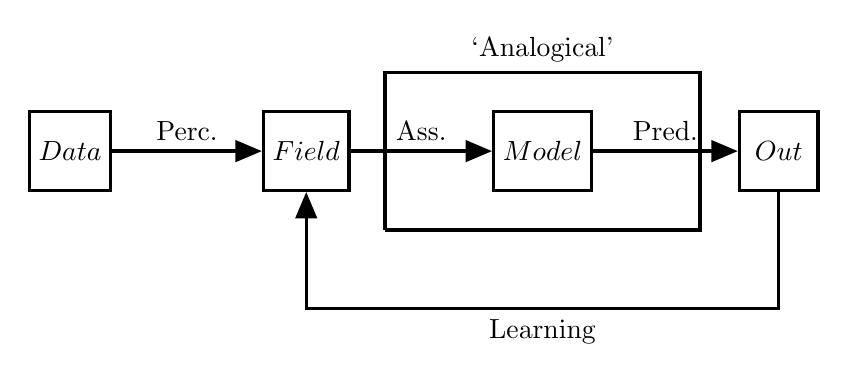
\begin{tikzpicture}[node distance=2cm]
\draw[very thick] (2,-1) -- (6,-1) -- (6,1) -- (2,1) node[midway,above] {`Analogical'} -- (2,-1);
\node (data) at (-2,0) [draw,very thick,minimum width=1cm,minimum height=1cm] {$Data$};
\node (syst) at (1,0) [draw,very thick,minimum width=1cm,minimum height=1cm] {$Field$};
\node (model) at (4,0) [draw,very thick,minimum width=1cm,minimum height=1cm] {$Model$};
\node (out) at (7,0) [draw,very thick,minimum width=1cm,minimum height=1cm] {$Out$};

% arrows
\draw [->,very thick] (data) -- (syst) node[midway,above]  {Perc.};
\draw [->, very thick] (syst) -- (model) node[midway,above] {Ass.};
\draw [->, very thick] (model) -- (out) node[midway,above] {Pred.};
\draw [->, very thick] (out) -- (7,-2) -- (1,-2) node[midway,below] {Learning} -- (syst);

\end{tikzpicture}
\caption{What has been referred to as analogical cognition may variously include parts of an associative mechanism, a cognitive system's internal model, and the application of that model for predictions and higher-order reasoning.  }

\end{center}
\end{figure}


[\dots]


In some of the first publications concerning transfer learning, transfer in neural networks is conceptualized as using the learned weights of a network at the outset---either directly or by using them as modulators to create other weights.  See for example \citet{Pratt1991,Pratt1993}.  Weights from a hidden layer to the output layer have also been shown to transfer classification capacity by \citet[p. 322]{Sharkeyetal1993}.  Modern deep ANNs have abundant hidden-to-hidden layer weights as well, and these are generally what are pre-trained in transfer learning techniques.  The input and output layers can be adjusted, but the largest number of transferred parameters are in the hidden layers.

%\begin{quote}
%In terms of connectionist research, adaptive generalization can be identified with the process by which a set of weights developed during the learning of one task is adapted for use on a second (novel) task.  The starting point for the second task can therefore be one of experience; its initializing weights incorporate the knowledge gained during training on the first task.  The question here then is one of understanding \emph{when} knowledge can be transferred between nets: identifying the circumstances under which pre-training on one task will assist (or interfere) with the performance of a subsequent task.  \cite[p. 314]{Sharkeyetal1993}
%\end{quote}

%Currently, an entry level data scientist does not need to train a new ANN for every task she encounters.  

With \texttt{keras}, a deep learning library for the Python programming language created by \citet{Chollet2015keras}, there are pre-trained deep networks (\emph{models}) available to be downloaded and used.  Similarly with \texttt{pytorch}.  These models are essentially sets of weights of certain dimensions, which have been trained on paradigmatic sets of data.  As an example, for image recognition, there are a number of models to pick off the shelf which have been trained on the ImageNet dataset from  \citet{Dengetal2009}.  This is a large dataset of images, and the models already have `experience' classifying the images in  this set.  These pre-trained models are useful for experimenting on new image data sets, and for when the number of data samples available on the new classification task are small.  Transfer learning is also making progress in other areas, such as natural language processing (NLP) with LSTMs.  Notably \citet{Ruderetal2018} recently introduced a method called Universal Language Model Fine-tuning which ``enables robust inductive transfer learning for any NLP task, akin to fine-tuning ImageNet models''.  The field is evolving rapidly, and perhaps future methods will involve some automated code writing from more generally capable models as well.  For example, Microsoft is using exclusive access to the GPT-3 model developed by OpenAI \citep{OpenAI_GPT-3} to translate natural language into code.


\subsection{EXCERPT: Bayesian Transfer (w/ Roland Poellinger)}

In briefly discussing the possibility of embedding such non-causal links into causal Bayes net structures, Verma and Pearl acknowledge the usefulness of such hybrid models:

\begin{quote}
The ability to represent functional dependencies would be a powerful extension from the point of view of the designer. These dependencies may easily be represented by the introduction of deterministic nodes which would correspond to the deterministic variables. Graphs which contain deterministic nodes represent more information than d-separation is able to extract; but a simple extension of d-separation, called D-separation, is both sound and complete with respect to the input list under both probabilistic inference and graphoid inference.  \cite[p. 75]{VermaPearlCausalNetworks1988} %\\\medskip
%
%D-separation is very similar to d-separation, only differing in that a path is rendered inactive by a set of nodes $Z$ under D-separation just\\in case it would be inactive under d-separation plus the case when a node on the path [\dots] is determined by $Z$.\\\medskip
\end{quote}

Symmetrical inter-theoretical relations like analogies are in our view a paradigm case study to implement such an extension.  We thus propose to model analogy as a relation between strictly correlated variables. It is  a non-causal and non-directional relation constructed on top of a syntactic isomorphism (formalized as a 1-1 function) in an extensions of a Bayes net causal model. Such hybrid structures have been discussed in philosophy  \citep{Poellinger2012}, as well as statistics (e.g., as chain graphs in \cite{Lauritzen01}).  We can extend a standard causal model triple $M=\langle U, V, F\rangle$ to a quadruple $\mathpzc{K}=\langle U, V, F, C\rangle$, where $U$ is a set of exogenous variables, $V$ a set of endogenous variables, $F$ a set of functional causal mechanisms (cf.  \cite[def. 7.1.1, p. 203]{Pearl2000}). The extension, $C$, is a set of \emph{epistemic contours}: a set of 1-1 functions $i_{j,k}$ that take the value of some variable $V_j$ and assign the value $i_{j,k}(V_j)$ to some other variable $V_k$ in the pattern. Importantly, intervening on one of these entangled variables will not break the contour.

Contours possess the properties we want for our analog relations. Yet, embedding entangled variables of this kind in Bayesian networks precisely renders them non-Markovian.\footnote{When Pearl claims that ``[t]he Markovian assumption [\dots] is a matter of convention, to distinguish complete from incomplete models''(Cf. \citep[p. 61]{Pearl2000} he naturally has Bayes net causal models (with distinct variables) in mind, which we just dismissed.} In the general case, the inferential framework must be tweaked to retain soundness,\footnote{For consistent reasoning and efficient computation of causal knowledge patterns to remain possible at all, acyclicity, independence (as expressed in the graphical \emph{d}-separation criterion), and the \emph{identifiability of causal effects} receive new explications. \cite{Poellinger2012} introduces a further graphical criterion, the \emph{principle of explanatory dominance}, to define under which conditions the Markov requirement can be reclaimed and extended Bayes nets can be utilized for causal inference.  
%Structure alone does not suffice for this task---more information is needed and comes in the form of intensional defaults and deviants as discussed, e.g., by Christopher \citet{Hitchcock2007}.
% By way of modifying the concept of \emph{identifiability of causal effects} it can be stated in which contexts which sub-portions of a partially directed graph support causal inference.
} but in our special case with a single intertheoretical bridge, we only require the idea of utilizing an undirected functional link to join two probabilistic chains (i.e., our two frames). So, how can we spell out analogical inference across this newly introduced bridge?

%Model nodes furthermore have an inner structure, where elements can be mapped onto each other in a unique way.  This means that on a more abstract level there is a one-one mapping between variables.
%[REF PEARL FUNCTIONAL RELATION FROM ROLAND's DISSERTATION]
%[QUICK INTRO TO CONTOURS MATH]



%\subsection{Analogical inference across symmetric links}\label{sec:application}

%In contrast to the general outline of epistemic contours above, analog contours are not generally transitive.  Thus, EC cliques will not be transitively closed.  [RIGHT?]  Just because $A::B$ and $B::C$ does not mean $A::C$.  Furthermore, we would not expect the same degree of confirmation to flow through such an informational link, although non-zero confirmation seems plausible enough to occur under certain circumstances.  That is, analogical contours will in general not fulfill these criteria, although there may be special cases that do.

In our proposal, the model-external postulate (or assumption, or also perception) ``$B_Q$ is similar to $B_F$ (in certain known respects)'' prompts the inclusion of a translation relation rather than the insertion of a new node. Analogical reasoning begins with a domain comparison which we characterize as the insertion of an inter-theoretical bridge.\footnote{This insertion can formally be understood as a structural mapping by which two frames are related.} Figure \ref{fig:SystemLadder} is a rendition of the Casimir effect example discussed above with the contour $i$ marking the analogical relationship between the frames at the level of systems $B_Q$ and $B_F$.

%\footnote{From now on we will omit the $\mathit{Aux}$ contributions in graphs, although the thorough reader may wish to keep them in mind.}

%\input{casimir-contour}

\begin{figure} [ht!]
\begin{center}
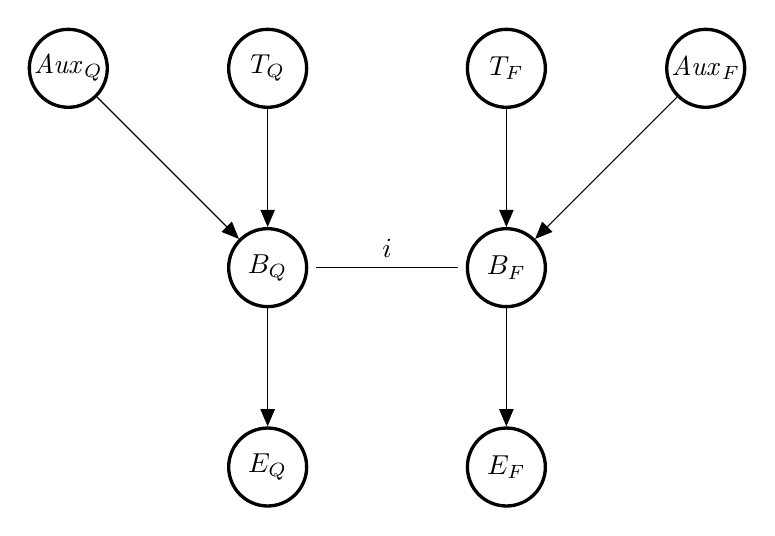
\begin{tikzpicture}[auto, node distance=5mm,
    latent/.style={circle,draw,very thick,inner sep=0mm,minimum size=10mm,align=center}]

\node[scale=0.99, latent] (X1) {$T_Q$};
\node[scale=0.99, latent, below=15mm of X1] (A) {$B_Q$};
\node[scale=0.99, latent, right=20mm of A] (B) {$B_F$};
\node[scale=0.99, latent, above=15mm of B] (X2) {$T_F$};
\node[scale=0.99, latent, below=15mm of A] (Y1) {$E_Q$};
\node[scale=0.99, latent, left=15mm of X1] (AUX1) {$\mathit{Aux}_Q$};
\node[scale=0.99, latent, right=15mm of X2] (AUX2) {$\mathit{Aux}_F$};
\node[scale=0.99, latent, below=15mm of B] (Y2) {$E_F$};
    \edge {X1} {A};
    \edge {X2} {B};
    \path[-,shorten >=1mm,shorten <=1mm] (A) edge node[midway]{$i$} (B);
    \edge {B} {Y2};
    \edge {A} {Y1};
    \edge {AUX1} {A};
    \edge {AUX2} {B};

 
\end{tikzpicture}
\caption{System-level analogy as epistemic contour $i$ with the intertheoretical bridge $i$ between $B_Q$ and $B_F$.}
\label{fig:SystemLadder}
\end{center}
\end{figure}












In this graph, the undirected edge between $B_Q$ and $B_F$, along with the formal explication we have introduced, provides a means for implementing analog confirmation as we have construed it.  A scientist or an artificial system can obtain $P(T_Q\,|\,E_F)>P(T_Q)$ while retaining the information represented by the undirected edge, and the ability at some later time to provide confirmation for $T_F$.  While in this case we might not need or want to confirm $T_F$, a general account \emph{should} provide for this.

One might wish to instead represent the analogical contour between $T_Q$ and $T_F$ (Figure \ref{fig:SystemLadder(STRONG)}).  However, this would be a much stronger claim since $B_Q$ and $B_F$ are determined to an additional extent by auxiliaries.  After all, confirmatory boosts in probability may be divided between the theory and auxiliary assumptions as per the Duhem-Quine problem.  An analogy at the theory level is, in some sense, an analogy that could be a step further towards unification than one at the system level.  

%We will return to briefly discuss (pre-)unification in Sec.\ \ref{sec:pre-unification}.

%\input{casimir-contour-strong}
\begin{figure} [ht!]
\begin{center}
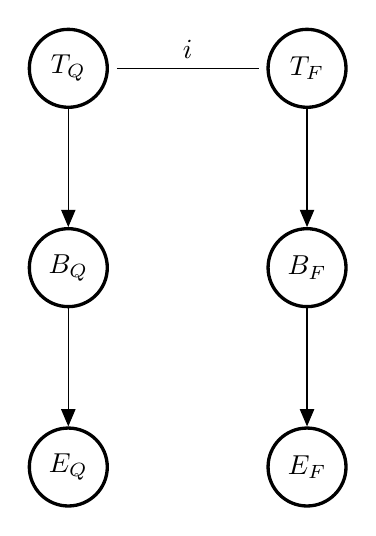
\begin{tikzpicture}[auto, node distance=5mm,
    latent/.style={circle,draw,very thick,inner sep=0mm,minimum size=10mm,align=center}]

\node[scale=0.99, latent] (X1) {$T_Q$};
\node[scale=0.99, latent, below=15mm of X1] (A) {$B_Q$};
\node[scale=0.99, latent, right=20mm of A] (B) {$B_F$};
\node[scale=0.99, latent, above=15mm of B] (X2) {$T_F$};
\node[scale=0.99, latent, below=15mm of A] (Y1) {$E_Q$};
\node[scale=0.99, latent, below=15mm of B] (Y2) {$E_F$};
    \edge {X1} {A};
    \edge {X2} {B};
    \path[-,shorten >=1mm,shorten <=1mm] (X1) edge node[midway]{$i$} (X2);
    \edge {B} {Y2};
    \edge {A} {Y1};

 
\end{tikzpicture}
\caption{Theory-level analogy as epistemic contour $i$ with the intertheoretical bridge $i$ between $T_Q$ and $T_F$.}
\label{fig:SystemLadder(STRONG)}
\end{center}
\end{figure}





















A potential option would also be to insert a collider structure between the model (system) levels representing an analogy.  However, as we have argued, granted analogies should not be represented as a node.  It is unclear what the content of the node would be, and the values it could take would arguably  depend upon a meta-level analysis of the network (i.e., it would be a self-referential node).  We think our approach of modeling the analogy as a functional relation is more consistent with the case study, as well as mathematically useful for future applications of the method.  Furthermore, there is support from the cognitive science literature treating analogy as an associative perceptual mechanism (i.e. structure mapping).  In this way, the transfer of knowledge from one domain to the other is \emph{direct}, not necessarily the result of a top-down generalization.  

%\marginal{Go through all possible ways of confirmation across c?}
%\marginal{collider would do it, but what is the content of the node? can only be meta-property of the network! should be relation.}

%emphasize that analogy is a structural transformation:
%
%Talk about relevance filter, sub-iso, analogy as structural transformation (based on meega)  vs node insertion, and confirmation across a theoretical bridge (not via switch node); remember Mark Colyvan's morphism through zigzag translation (as a process towards isomorphism!?) %Use Godehard Link, CoLo pp. 398 ff.

%\subsection{Translation via relevant sub-isomorphisms}\label{sec:sub-iso}

We take analog contours to be an expression of a modeling relationship between frameworks.  It can be thought of formally as a translation relation based on a \emph{relevant sub-isomorphism}, which has been anticipated in the literature on models and representations in science, cf.\ \cite{SEP2012}:

%\footnote{We have included in our bibliography the complete references cited in this quote for completeness.}

\begin{quote}
%Although this question is not explicitly addressed in the literature on the so-called semantic view of theories, some answers seem to emerge from its understanding of models. 

One version of the semantic view, one that builds on a mathematical notion of models, posits that a model and its target have to be isomorphic (van \cite{vanFraassen1980}; \cite{Suppes2002}) or partially isomorphic (Da \cite{DaCostaetal2003}) to each other. Formal requirements weaker than these have been discussed by \cite{Mundy1986} and \cite{Swoyer1991}. Another version of the semantic view drops formal requirements in favor of similarity (\cite{Giere1988,Giere2004}; \cite{Teller2001}). This approach enjoys the advantage over the isomorphism view that it is less restrictive and also can account for cases of inexact and simplifying models. However, as Giere points out, this account remains empty as long as no relevant respects and degrees of similarity are specified. The specification of such respects and degrees depends on the problem at hand and the larger scientific context and cannot be made on the basis of purely philosophical considerations (\cite{Teller2001}).
\end{quote}

\nocite{vanFraassen1980}
\nocite{Suppes2002}
\nocite{DaCostaetal2003}
\nocite{Mundy1986}
\nocite{Swoyer1991}
\nocite{Giere1988}
\nocite{Giere2004}
\nocite{Teller2001}


We follow this line of reasoning and formulate a relevance filter in order to capture the purpose-driven selection of theoretical entities to be translated. Of course, basing analogy on a purpose-driven relevance concept makes the concept of analog models context-specific.  The important point is that there is \emph{some} structural relationship which is mapped between the model and target systems.  We can embrace this and call $B_F$ an analog model of $B_Q$ \emph{relative to}

\begin{enumerate}
\item a relevance filter $Rlv$;
\item a bijection between the relevant properties of $B_Q$ and $B_F$ (an isomorphism between sub-structures of $B_Q$ and $B_F$).
\end{enumerate} 

The filter function $Rlv$, an indicator function over the descriptive elements of both frameworks, selects for each semantic category (for individual objects and each set of n-ary relations between such objects) subsets of equal magnitude; i.e., for each category:

\begin{equation}
||\,Rlv(B_Q)\,|| = ||\,Rlv(B_F)\,||\,.
\end{equation}

%For relevant properties $P$ and object vectors $\mathbf{x}$ of a given framework, the translation function (or: interpretation) $i$ bijectively translates objects and sets of objects into a second framework; for $P_Q = i(P_F)$ and $\mathbf{x}_Q = i(\mathbf{x}_F)$:

If $B_Q$ and $B_F$ behave alike with respect to relevant parts (i.e., parts selected by $Rlv$) that are described by $P_Q \mathbf(x)_Q$ and $P_F \mathbf(x)_F$ (with properties $P$ of objects $x$ in the respective models), then the following formula explicates the analog relation between frameworks via translation $i$:

\begin{equation}
\forall P_F, \mathbf{x}_F (P_F(\mathbf{x}_F) \leftrightarrow P_Q(\mathbf{x}_Q) )\,.
\end{equation}

Note that this isomorphism might be the result of iteratively fine-tuning non-bijective translations between the frameworks.%\footnote{We are thankful to Mark Colyvan for valuable discussions about the nature of this morphism.}

Having defined the propagation of information across the epistemic contour in this way, tracing confirmatory support in Fig.\ \ref{fig:SystemLadder} yields the following:
\begin{eqnarray}
P(B_F \,|\, E_F ) > P(B_F)\label{eq:fluidEvidence}\\
P(T_Q \,|\, B_Q ) > P(T_Q)\label{eq:quantumSystem}\\
P(i(B_F) \,|\, B_F ) > P(i(B_F))\label{eq:contour}
%\item $P(B' | T_Q ) > P( B' )$
%\item $P(T_{Q} | B' ) > P( T_{Q} )$
\end{eqnarray}
where $i(B_F)$ represents specific information about the properties of $B_Q$ relevant for the analogical inference (i.e., as chosen by the filter function). Eq.\ \ref{eq:contour} exploits the characterization of contour $i$ as 1-1 function: Learning $B_F$ tells us more about the $Rlv$-selected properties and objects at the core of $B_Q$, thereby raising our degree of belief in those $B_Q$ that are compatible with $i(B_F)$. Now, by transitivity, \ref{eq:fluidEvidence}, \ref{eq:quantumSystem}, and \ref{eq:contour} together entail
\begin{equation}
P(T_Q \,|\, E_F ) > P(T_Q),\label{eq:contourconfirmation}
\end{equation}
which was implied by our list of desiderata above.  Formula \ref{eq:contourconfirmation} is an instance of Bayesian confirmation---this time across theoretical frameworks, though, and it encodes what we set out to achieve: Bayesian confirmation from an analog model.

%\footnote{As soon as one learns of a specific instantiation of $i(B_F)$, i.e., the relevant core of $B_Q$, those theoretical entities not in the $Rlv$ mapping must be updated in line with consistency requirements.}


\section{Deep Learning Internship at Cray, Inc.}

\noindent Cray, now part of Hewlett Packard Enterprise,  manufactures supercomputers. They also provide high performance software to help customers like national scientific labs deploy jobs onto petascale and exascale compute clusters. \\

\noindent I worked with Cray's Distributed Deep Learning Plugin team. The plugin is a simple wrapper to modify python machine learning scripts to work across GPU clusters, using MPI (e.g. AllReduce) to communicate gradients between threads and average them.  I applied, tested, and experimented with the Plugin across multiple GPUs (gradient averaging using MPI), on a variety of ANN architectures including: LSTM, CNN, CapsNet, and Deep RL/DQN.  The latter was the most sophisticated, and should have been prioritized since I ended up running out of time before the plugin was functional on a deep reinforcement learning model. \\

\noindent \textbf{What I Used:} Python, Jupyter, Slurm, SSH onto \faLinux \  Linux GPU clusters, Keras, Anaconda, Bash, Git.  I mainly used Keras, scheduled jobs via Slurm, managed ML/DL packages and versions with Anaconda and pip, and committed code to internal git repos. \\

\noindent \textbf{What I Learned:}  Parallelization (MPI) through distributing computation to threads and communicating between them.  Initiation task for me was to estimate pi with a Monte Carlo simulation in Fortran.  \\

\noindent \textbf{Example Code Repo:} \href{https://github.com/CameronBeebe/Monte_Carlo}{Monte Carlo calculating pi with MPI and pyspark}







\section{Project: RL in Agent Based Modeling (Netlogo)}

Coding project in agent based modeling course at the MCMP using the Netlogo programming language.  I modified a simple reinforcement learning agent-based model to include a mechanism of ``forgetting''.  Years later I would describe the project as  utilizing a form of dropout. \\

\noindent \textbf{What I Learned:} Polya Urn as simple model of Reinforcement Learning (changing probability distribution of ``balls'' (actions) in an urn).  Noise as a regularizer. \\

\noindent \textbf{Full Paper:} \href{https://www.researchgate.net/publication/321228909_Modeling_Memory_in_Signaling_Games_Deep_and_Surface_Forgetting}{Modeling Memory in Signaling Games: Deep and Surface Forgetting}







\section{Academic environment and relevant courses in Math and AI}

Most courses I took involved math, programming, and formal methods to varying degrees at the Munich Center for Mathematical Philosophy (MCMP) and Graduate School of Systemic Neurosciences (GSN).  \\

\noindent The philosophy curriculum at the MCMP required basic formal methods: probability theory, information theory, formal logic, and basic linear algebra and calculus if working in more technical areas in philosophy of physics and interdisciplinary AI theory.  \\

\noindent Formal epistemology, rationality, and other philosophical aspects of cognition in consideration of artificial systems. \\

\noindent Some of the courses included: \\

Weekly Neurophilosophy seminars, Machine Epistemology (Wheeler), Rationality (Roy), The Unity and Plurality of Cognitive Science, Statistical Modeling and Data Analysis (Leibold), Philosophy of Probability (Mayo-Wilson), Quantum Information and Entanglement (Paredes), Philosophy of Quantum Computation (Cuffaro)\dots


\section{Coding}

I have the most experience with python and associated packages and tools.  I have used jupyter notebooks, pandas, scikit-learn, keras (and some tensorflow through tf.keras), and other related packages.  Before I got into python I also used Netlogo (a language specialized for agent based modeling and visualization), some octave and matlab, and I am comfortable working through the command line on linux/unix terminals.  In general, I am able to read and write code and learn new syntax if I have to.  

\section{Real World Data Experience}

For the last year and a half I have been working at a cultivation facility start up in Nederland, Colorado.  As we are a small team, most of us do everything.

\begin{multicols}{2}
\begin{itemize}
    \item \textbf{Measurement and Recording}: PH; total dissolved solids (tds) or parts per million (ppm); water temperature; room humidity and temperatures; nutrient solution amounts; plant waste weight; 
    \item \textbf{Calibration}: PH and TDS measurement devices.
    \item \textbf{Measurement:} 
    \item \textbf{Preparation:} Mixing nutrients
\end{itemize}
\end{multicols}

\section{Other Experience}

\begin{multicols}{2}
\begin{itemize}
\item PyData talk on Transfer Learning
\item Nano degree Deep Learning (Udacity)
\item Talk at HLRS Stuttgart on Ashby's Cybernetics and characterizing ANNs as cybernetic regulators.
\item ML Reading Group at MCMP (Sterkenberg)
\item Outreach: talk about ChatGPT at local library.
\end{itemize}
\end{multicols}

\bibliographystyle{apacite}
\bibliography{MyBibliography1}


\end{document}  